% The topic
  % Reality
  % Data
  % Interpretation
  % Bias
% The course
  % Essentials
  % Mechanics
  % Homework
  % Logistics
% Notes
  % On computers
  % On software
  % On slides
  % On emails
% Coursework

\documentclass[t]{beamer}
\usetheme{hkllite}

\title{introduction}
	\author{François Briatte \& Ivaylo Petev}
	\date{Week~\#1}

\begin{document}

  \frame[plain]{
		\titlepage\\[7.25em]
		\begin{columns}[T]
			\column{.50\textwidth}
				\tableofcontents[hideallsubsections]
			\column{.35\textwidth}
				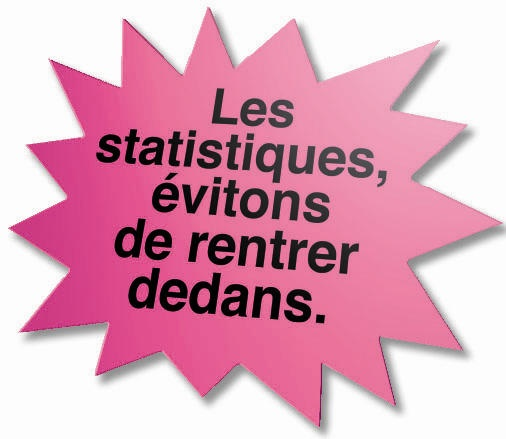
\includegraphics[width=\textwidth]{stats-evitons}
		\end{columns}
	}
	%
	%
	
	%
	%
	\section{The topic}
	%
	%
	
  % 
  %
  \subsection{Reality}
  %
  %
  
  \begin{frame}[t]{Reality is \red{predictable}}
    \href{http://articles.latimes.com/2010/aug/21/local/la-me-predictcrime-20100427-1}{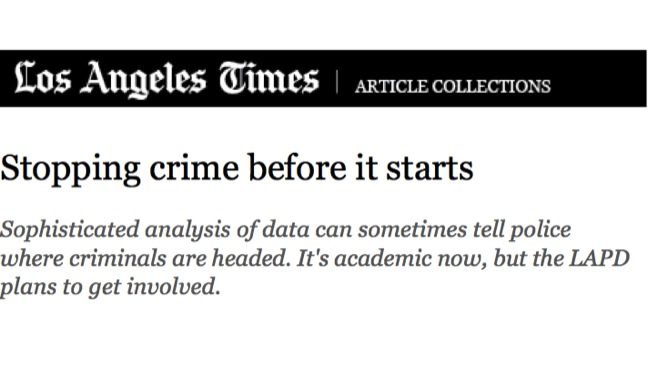
\includegraphics[width=\textwidth]{predicting}}
  \end{frame}
  %
  %
    
  \begin{frame}[t]{Reality is \red{visualizable}}
    \href{http://www.bricoleurbanism.org/whimsicality/urban-fabric-form-comparison/}{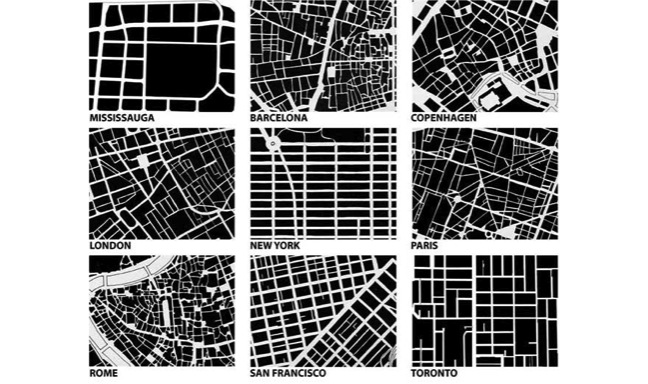
\includegraphics[width=\textwidth]{visualize}}
  \end{frame}
  %
  %
  
  \begin{frame}[t]{Reality is \red{multidimensional}}
    \href{http://www.last.fm/user/phnk1/library}{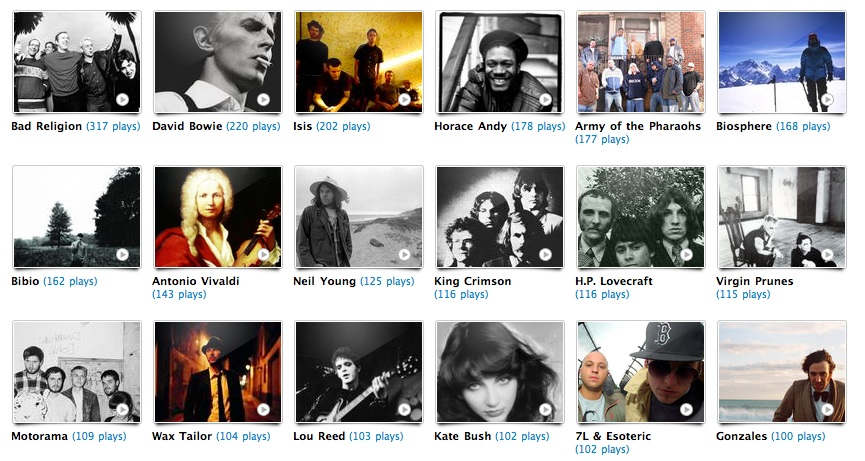
\includegraphics[width=\textwidth]{lastfm}}
  \end{frame}
  %
  %

  \begin{frame}[c]{Reality is \red{relational}}

    \begin{columns}[T]

      \column{.45\textwidth}

      \begin{center}
        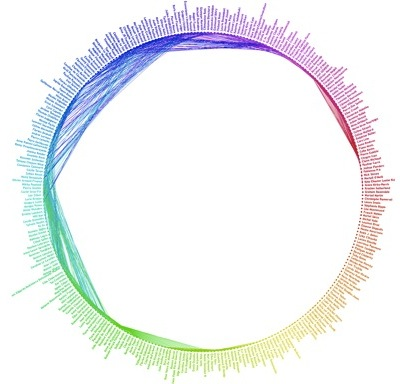
\includegraphics[height=4cm]{friendwheel}\\
        \vspace{0.74cm}
        Friendship ties on Facebook
      \end{center}

      \column{.45\textwidth}

      \begin{center}
        \href{http://www.sociology.columbia.edu/pdf-files/bearmanarticle.pdf}{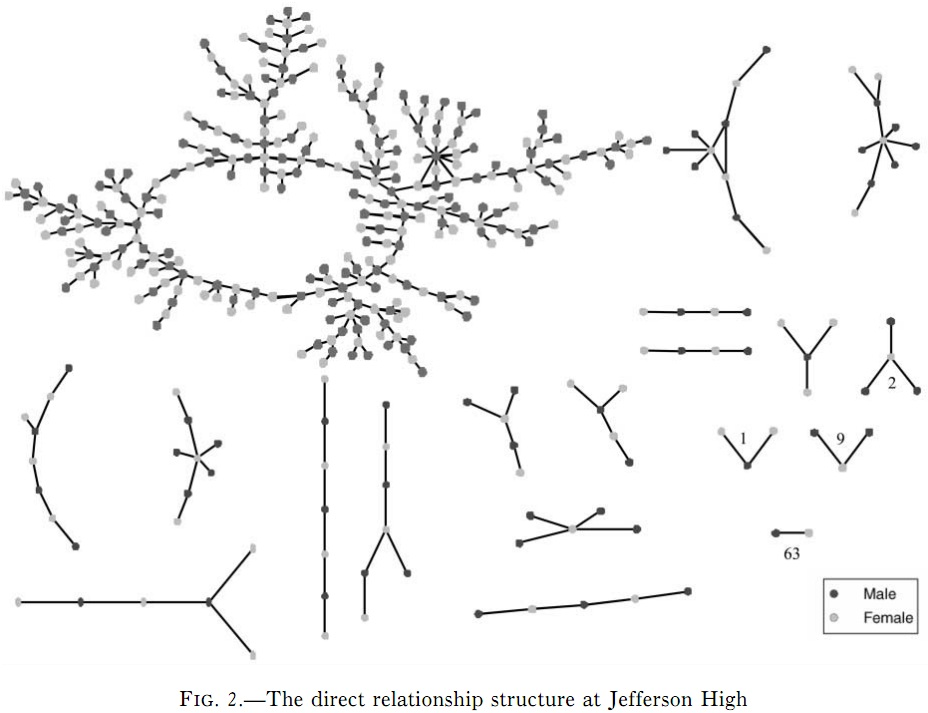
\includegraphics[height=4cm]{network}}\\
        \vspace{0.7cm}
        Sexual ties in high school
      \end{center}

    \end{columns}

  \end{frame}
  %
  %
  
  %
  %
  \subsection{Data}
  %
  %
  
  \begin{frame}[t]{Data stand as \red{professional assets}}
    
\includegraphics[width=\textwidth]{oecd}
  \end{frame}
  %
  %
  
  \begin{frame}[c]{Data stand as \red{policy expertise}}

    \begin{center}
      \href{http://www.securite-sociale.fr/chiffres/ccss/notesconj/conj200903.pdf}{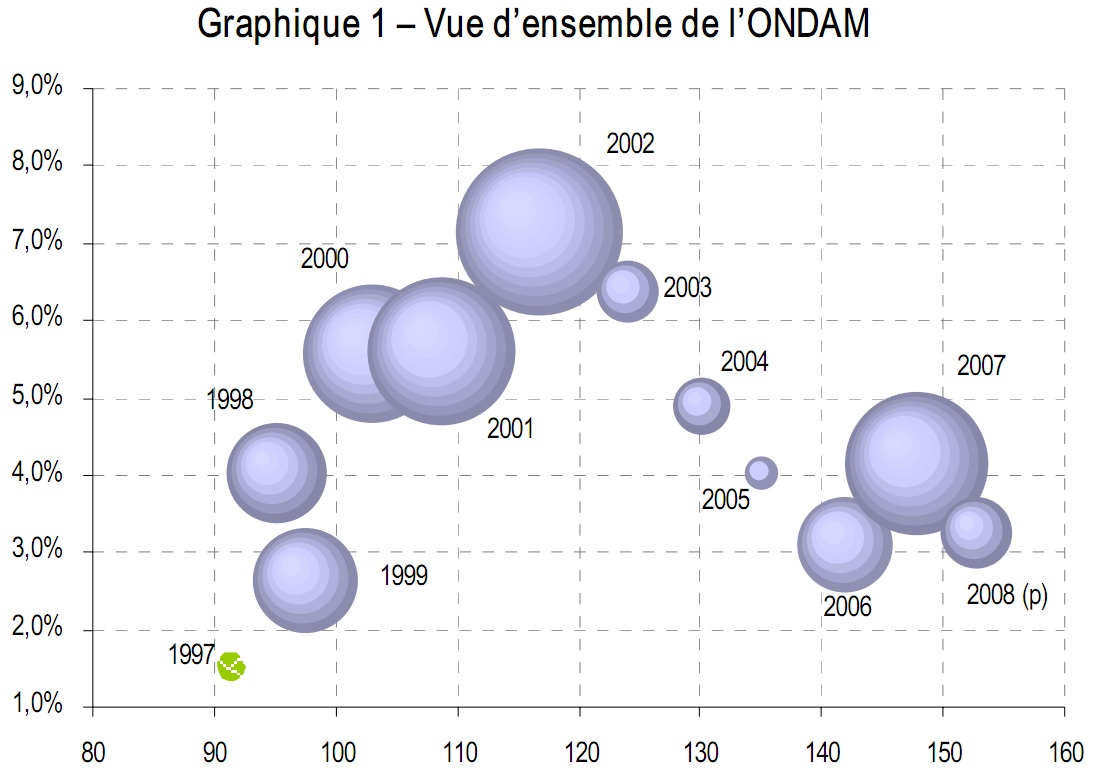
\includegraphics[width=.75\textwidth]{ondam}}
    \end{center}    

  \end{frame}
  %
  %
  
  %
  %
  \subsection{Interpretation}
  %
  %
  
  \begin{frame}[c]{\red{Interpretation} is key to all analysis}

    \begin{columns}[T]
      
      \column{.45\textwidth}

      \begin{center}
        \href{http://jhfowler.ucsd.edu/alone_in_the_crowd.pdf}{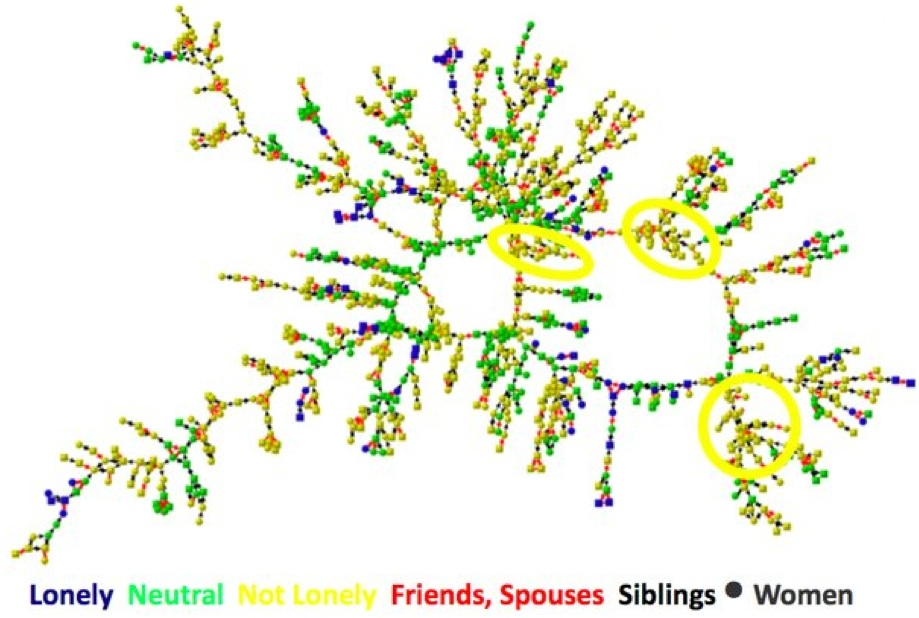
\includegraphics[height=4cm]{fowler-network}}\vspace{1cm}
        Loneliness in social networks
      \end{center}
      
      \column{.45\textwidth}

      \begin{center}
        \href{http://books.google.fr/books?id=gvgCYyFN7RIC&pg=PA19&lpg=PA19}{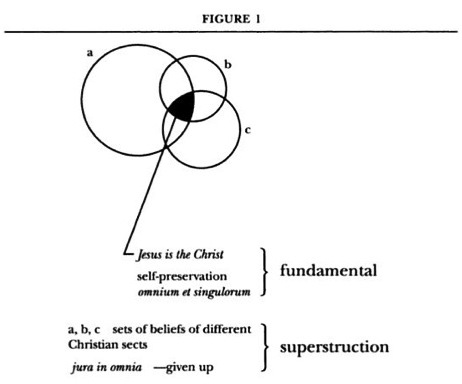
\includegraphics[height=4cm]{jesus}}\vspace{1.05cm}
        Sets of Christian beliefs
      \end{center}
      
    \end{columns}

  \end{frame}
  %
  %
  
  \begin{frame}[c]{\red{Interpretation} is difficult}

    \begin{columns}[T]

      \column{.45\textwidth}

      \begin{center}
        \href{http://jhfowler.ucsd.edu/alone_in_the_crowd.pdf}{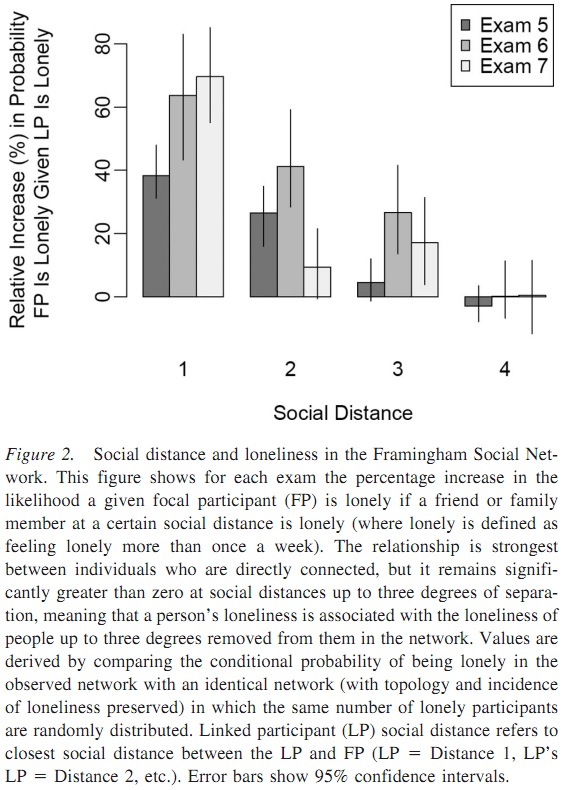
\includegraphics[height=5cm]{fowler-social-distance}}\\
        \vspace{0.25cm}
        With explanation
      \end{center}

      \column{.45\textwidth}

      \begin{center}
        
\includegraphics[height=5cm]{explain}\\
        \vspace{0.25cm}
        Without explanation
      \end{center}

    \end{columns}     

  \end{frame}
  %
  %
  
  \begin{frame}[t]{\red{Interpretation} is what this course is eventually about}
    
    \begin{center}
      \href{http://www.phdcomics.com/comics.php?f=1219}{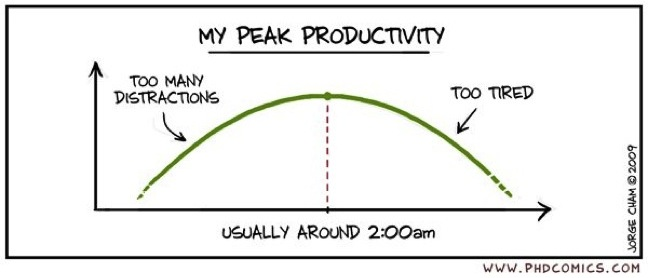
\includegraphics[width=.8\textwidth]{phdcomics-productivity}}
    \end{center}
    
    \begin{exampleblock}{Questions}

      \begin{itemize}
        \item What is the \textbf{measurement} method for each axis?
        \item What is the \textbf{probability} of 2am being the cutoff point?   
        \item What is the \textbf{shape} of the time/productivity relationship?
      \end{itemize}

    \end{exampleblock}
    
  \end{frame}
  %
  %
  
  %
  %
  \subsection{Bias}
  %
  %
  
  \begin{frame}[t]{\red{Bias} and measurement}
    
    \begin{block}{Observational data}

      \begin{itemize}
        \item Survey design
        \item Sampling strategy
        \item Question wording
      \end{itemize}
    
    \end{block}

    \begin{block}{Official statistics}
    
      \begin{itemize}

        \item Unreliable aggregates       % e.g. GDP in China
        \item Low statistical capacity    % e.g. "Poor Numbers" in Africa
				\item Ecological fallacies				% lack of granularity

      \end{itemize}

    \end{block}
        
  \end{frame}
  %
  %
  
  \begin{frame}[t]{\red{Bias} and manipulation}

    \begin{columns}[T]
      
      \column{.3\textwidth}

      \begin{itemize}
        \item Media coverage        % e.g. climate change
        \item Political spin        % e.g. unemployment and educational achievement in France
        \item Policy implications   % e.g. deficit figures and the IMF bailout in Greece
      \end{itemize}
      
      Add to that:
      
      \begin{itemize}
        \item \href{http://andrewgelman.com/2012/08/scientific-fraud-double-standards-and-institutions-protecting-themselves/}{scientific fraud},
        \item \href{http://andrewgelman.com/2012/10/ethical-standards-in-different-data-communities/}{data ethics}, % or lack thereof
        \item \href{https://en.wikipedia.org/wiki/Merchants_of_Doubt}{doubt-mongering}, % and the market for skepticism
        \item publishing bias, … % in journals and clinical trials
      \end{itemize}
              
      \column{.6\textwidth}
        
        \href{https://metofficenews.wordpress.com/2010/07/28/unmistakable-signs-of-a-warming-world/}%
        {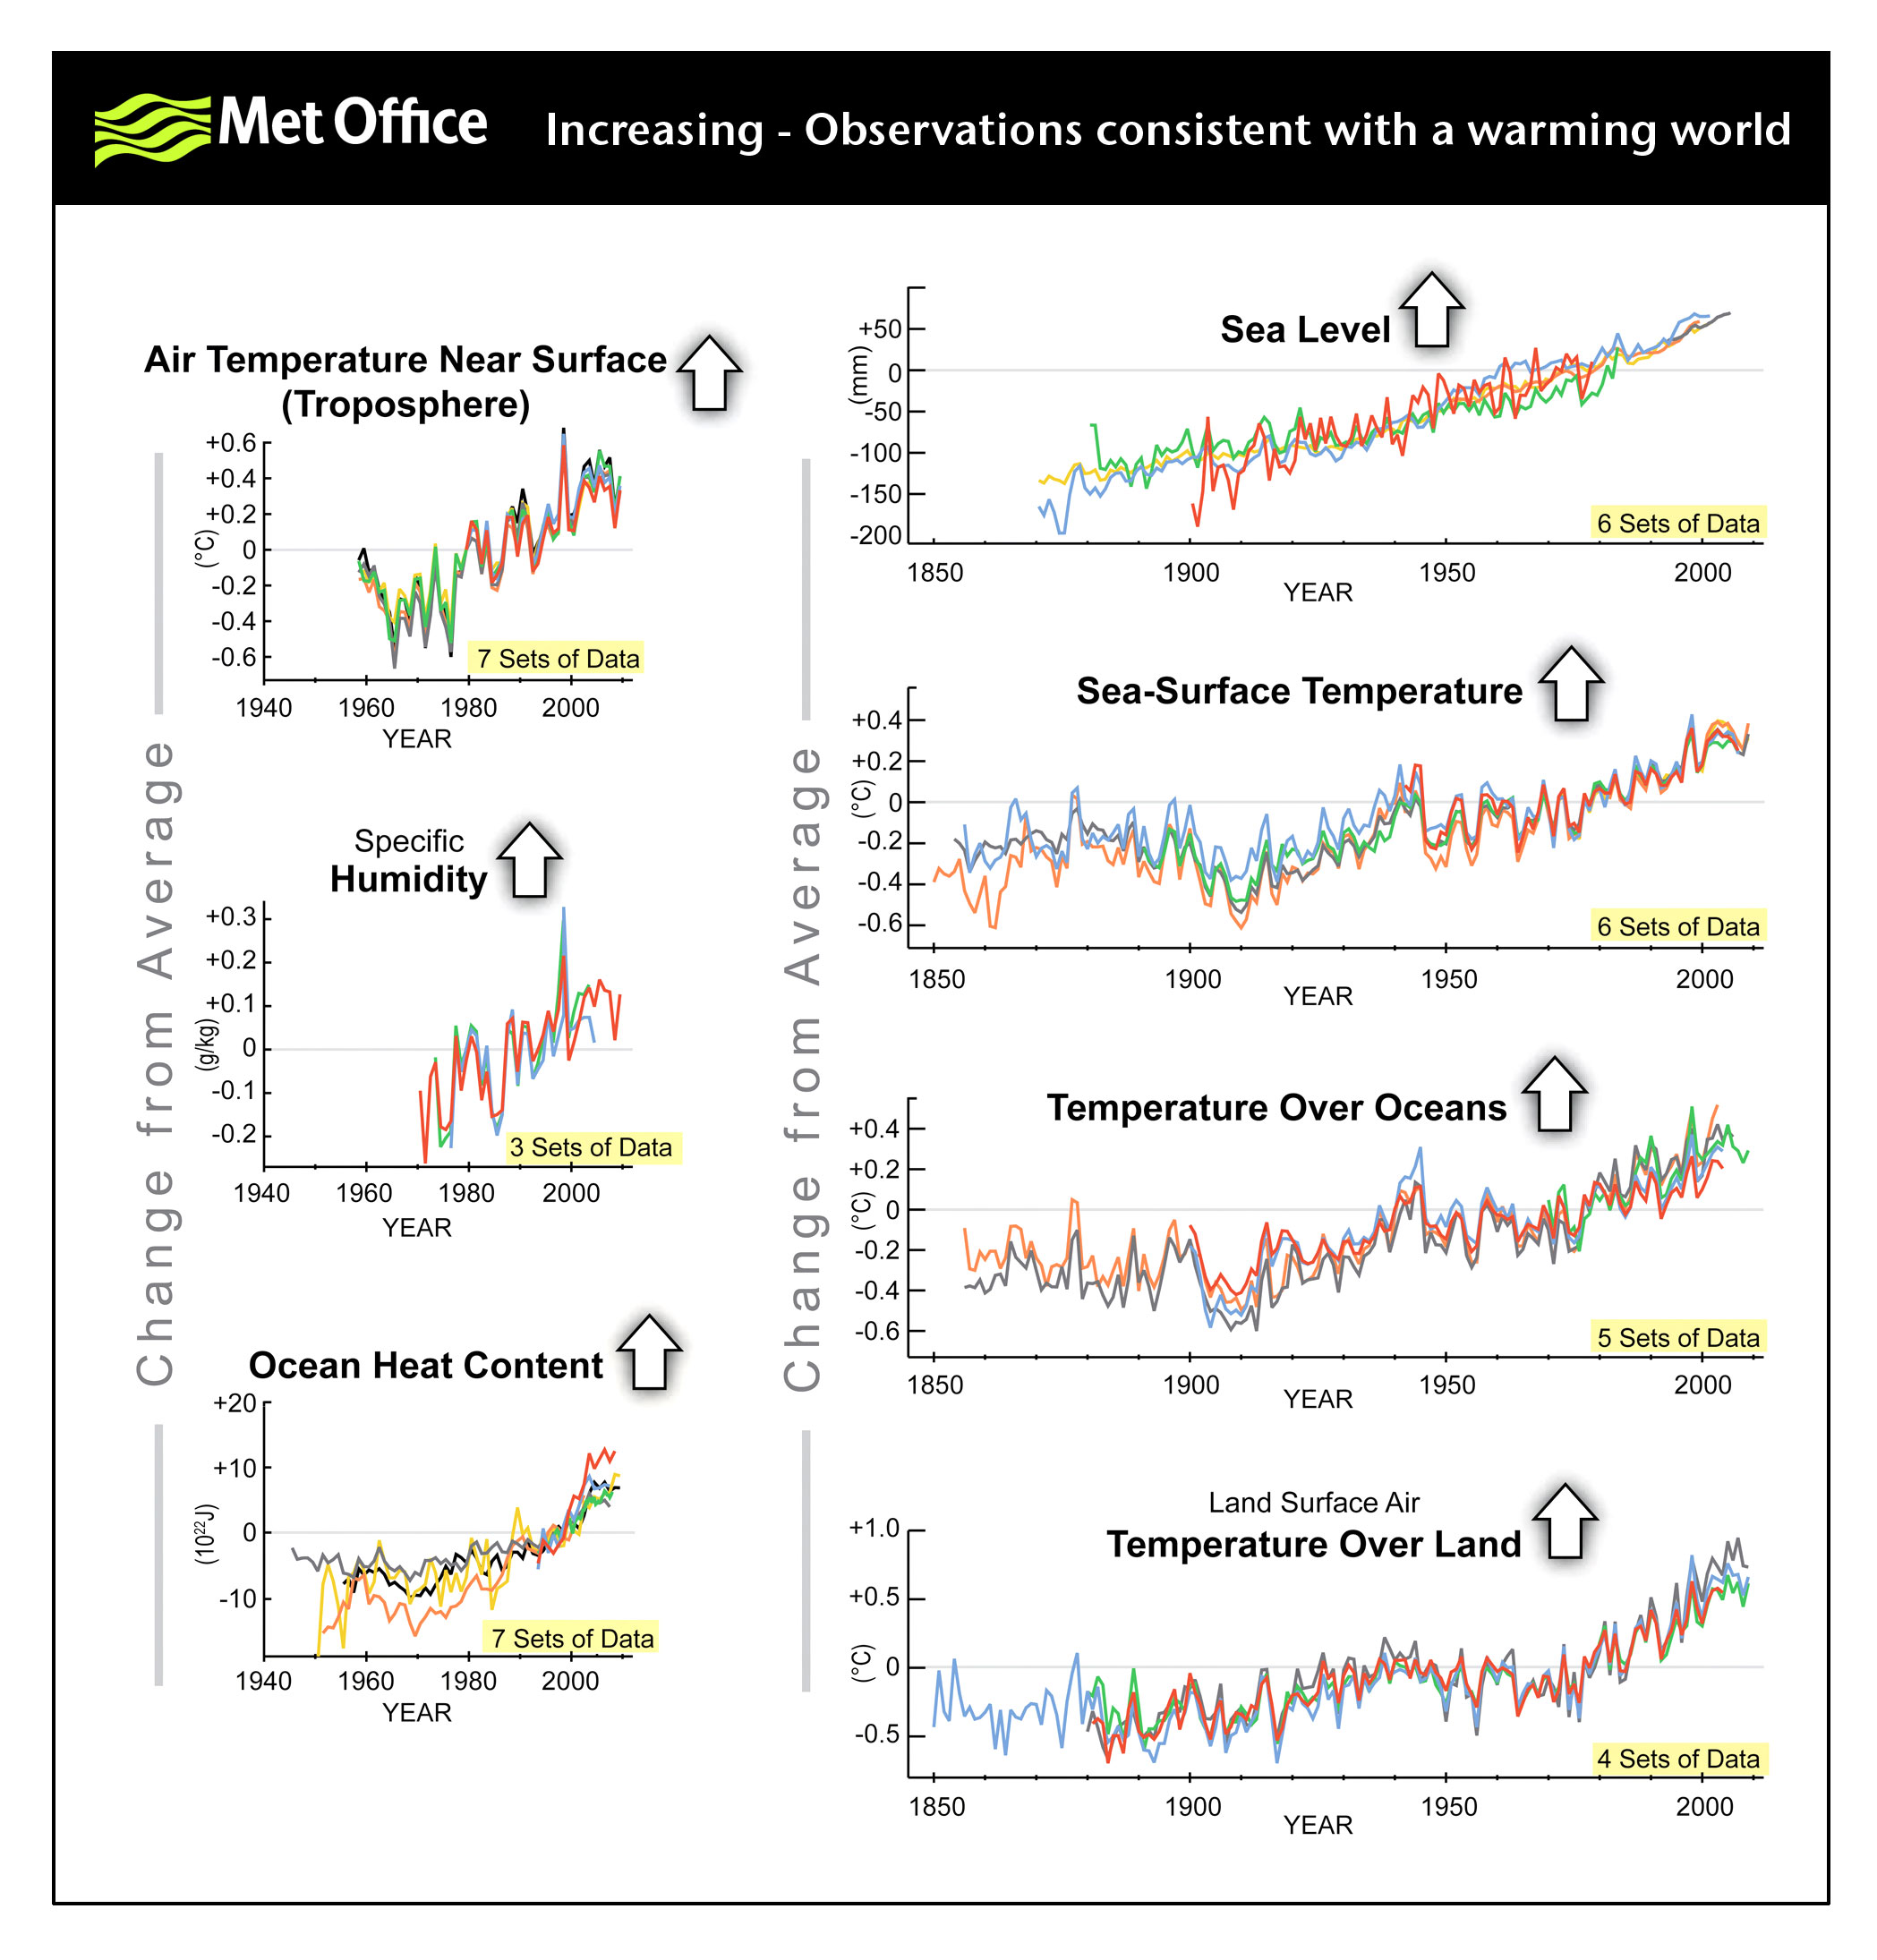
\includegraphics[width=.9\textwidth]{warming}}

    \end{columns}
    
  \end{frame}
  %
  %
    
  \begin{frame}[c, plain]
    
    \href{http://www2.psych.ubc.ca/~henrich/pdfs/WeirdPeople.pdf}{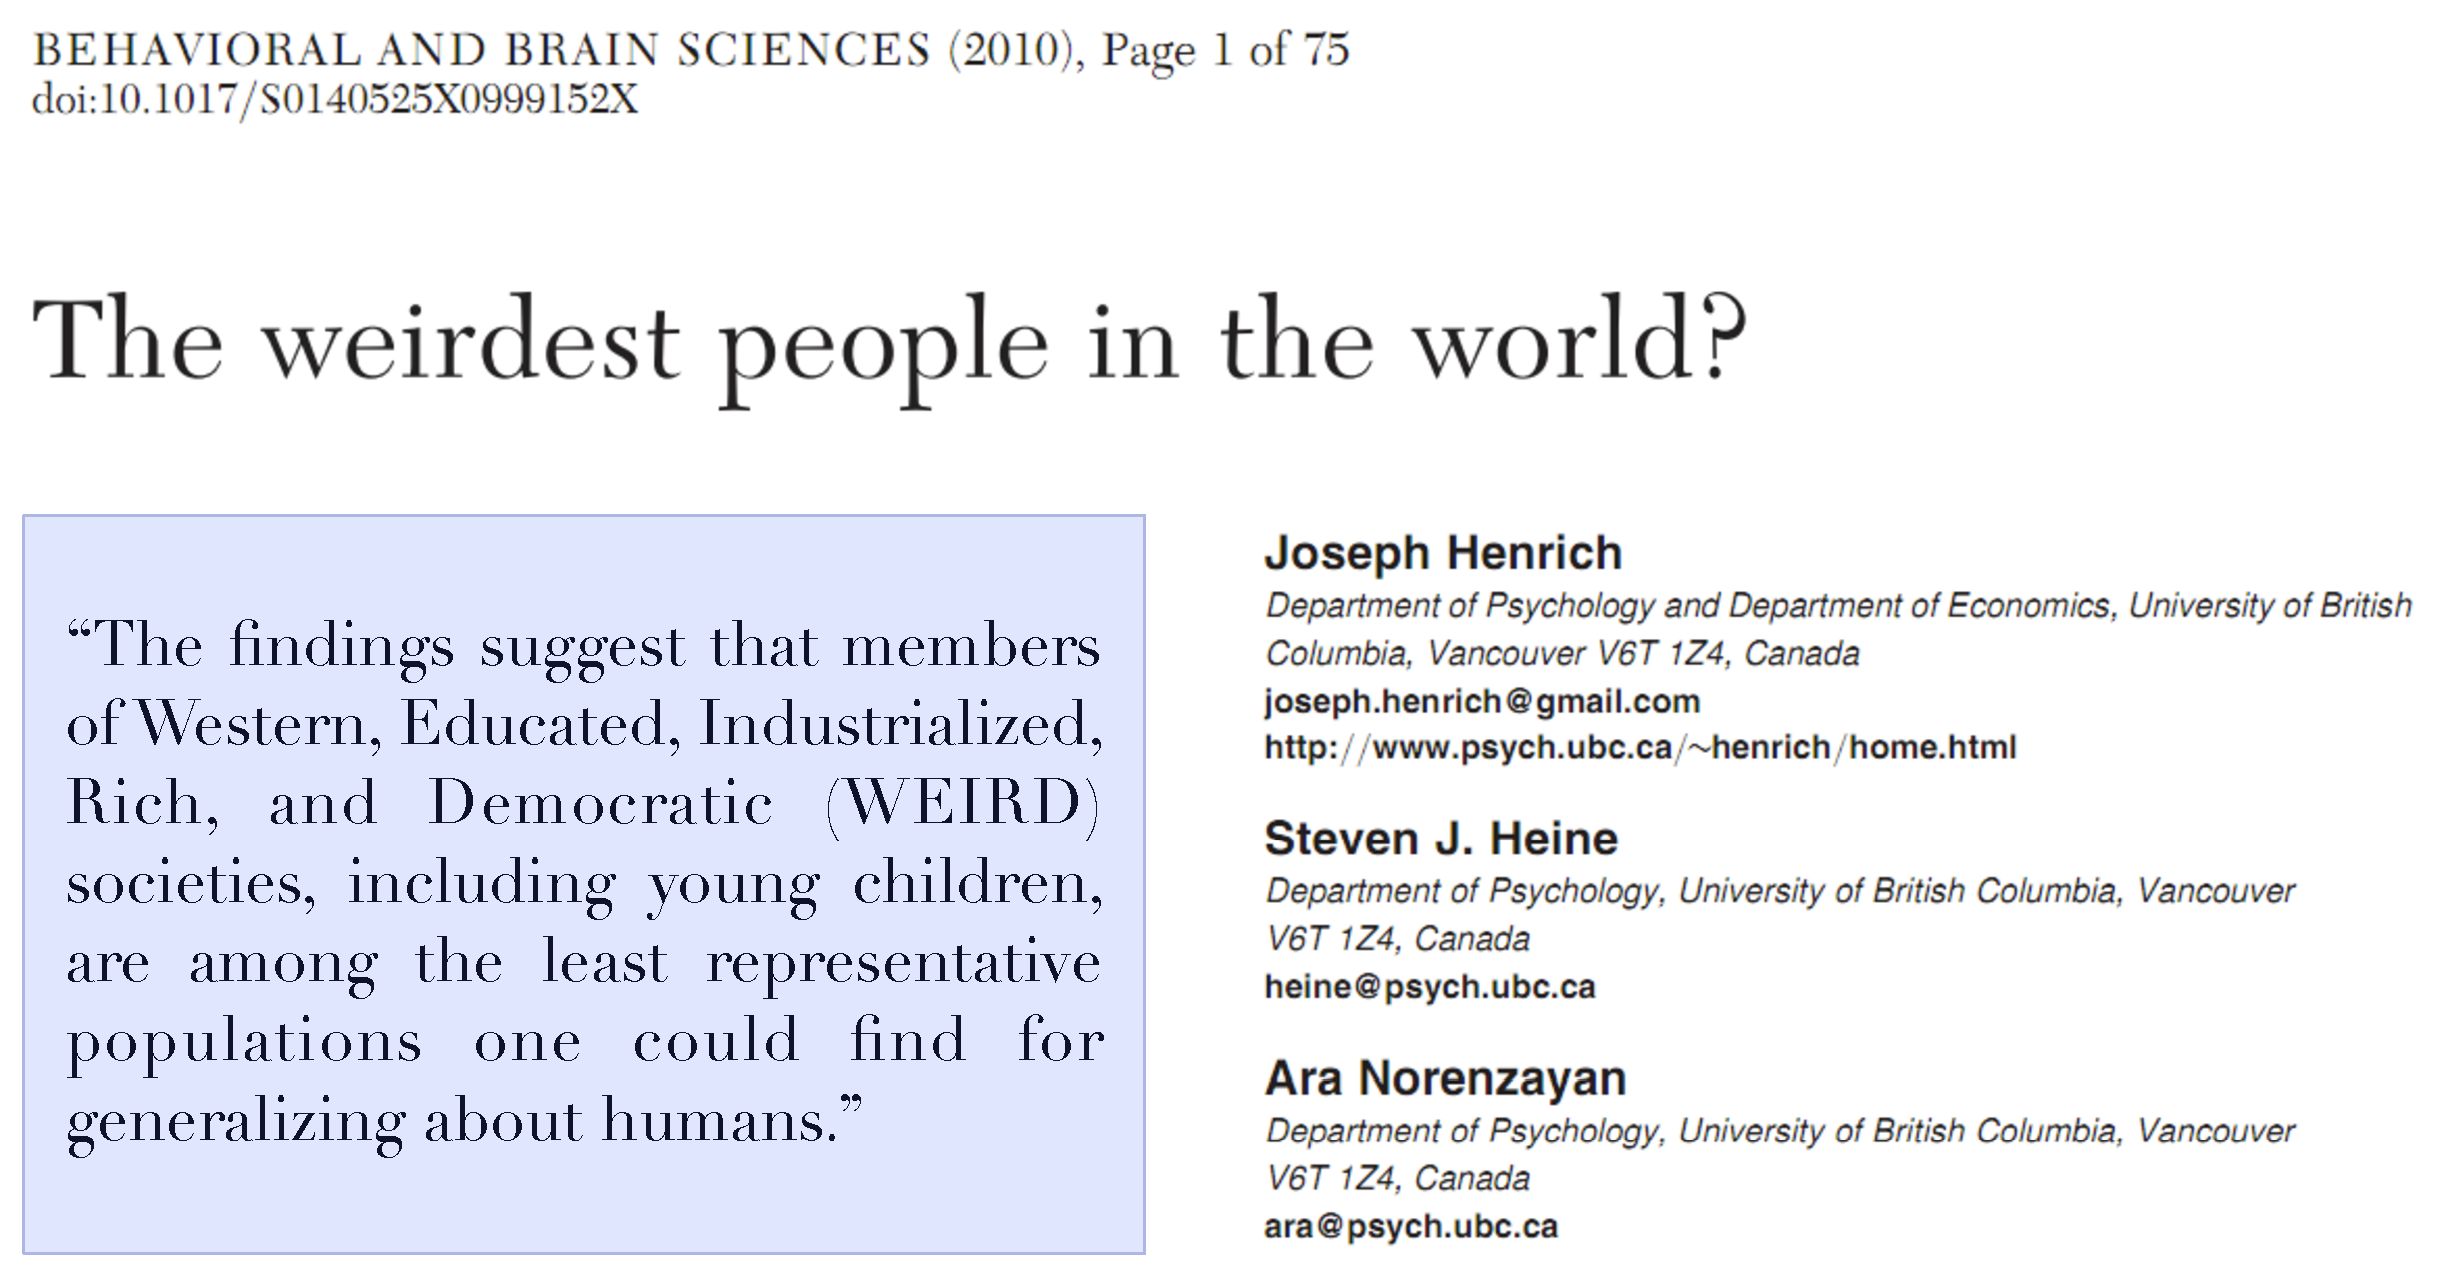
\includegraphics[width=\textwidth]{bbs.pdf}}  

  \end{frame}
  %
  %

% \href{https://en.wikipedia.org/wiki/The_Incredulity_of_Saint_Thomas_(Caravaggio)}%
      {}
  \begin{frame}[c, plain]{}
    \absoluteimage{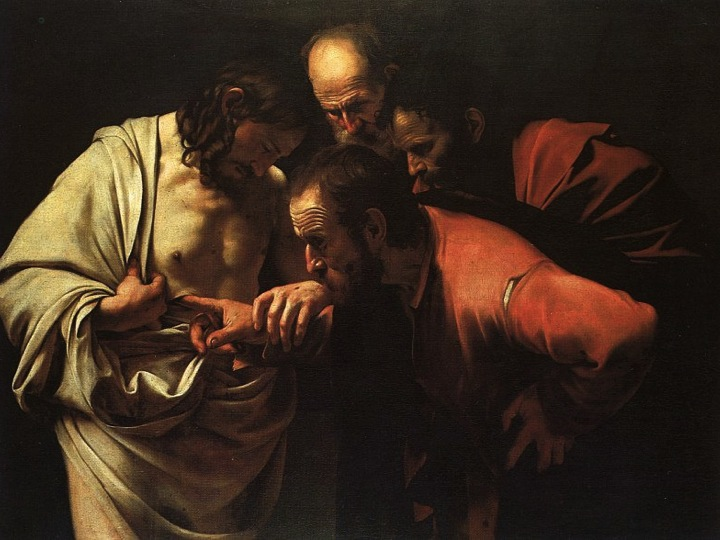
\includegraphics[width=\paperwidth]{caravaggio}}
  \end{frame} 
  %
  %
  
	%
	%
  \section{The course}
	%
	%
	
  % 
  %
  \subsection{Essentials}
  %
  %
  
  \begin{frame}[t]{Course \red{essentials}}

    \begin{block}{Core learning objectives}
      \begin{enumerate}
        \item Data management
        \item Statistical estimation
        \item Regression modelling
      \end{enumerate} 
    \end{block}
  
    \begin{block}{Core teaching blocks}
      \begin{itemize}
        \item Statistical theory      \hfill … textbook \textbf{readings}
        \item Statistical computing   \hfill … Stata do-files (\textbf{code})
        \item Tons of social science  \hfill … example \textbf{papers}
      \end{itemize}   
    \end{block}
    
  \end{frame}
  %
  %

  % 
  %
  \subsection{Mechanics}
  %
  %
	
  \begin{frame}[t]{Course \red{mechanics}}

  \begin{columns}[T]

    \column{.5\textwidth}

    \begin{block}{Requirements}
      \begin{itemize}
        \item Attendance
        \item Homework
        \item No plagiarism
      \end{itemize}
    \end{block}
  
    \begin{alertblock}{Grading}
      \begin{itemize}
        \item Code and paper
        \item Draft, revised, final
        \item Project management
      \end{itemize}
    \end{alertblock}

      \column{.4\textwidth}

    \begin{center}
      
\includegraphics[width=\textwidth]{due-tomorrow}\vspace{1em}
      
      This won't work.
    \end{center}

  \end{columns} 
    
  \end{frame}
  %
  %

  % 
  %
  \subsection{Homework}
  %
  %
  
  \begin{frame}[t]{Course \red{homework}}

    % \begin{exampleblock}{Course website} 
    %     \url{http://f.briatte.org/teaching/quanti/}
    % \end{exampleblock}
    
    \begin{block}{Readings}
      \begin{itemize}
        \item Urdan 								\hfill … essential textbook
        \item Feinstein and Thomas  \hfill … details on modelling
        \item Stata Guide           \hfill … practical walkthrough
      \end{itemize} 
    \end{block}
  
    \begin{block}{Coursework}
      \begin{itemize}
          \item \textbf{Replicate} the weekly do-files
          \item \textbf{Code} your own data analysis
          \item \textbf{Write} an empirical research paper
      \end{itemize} 
    \end{block}
    
  \end{frame}
  %
  %
  
  % 
  %
  \subsection{Logistics}
  %
  %
	
  \begin{frame}[t]{Course \red{logistics}}

    \begin{columns}[T]

      \column{.35\textwidth}
      
        \textbf{Elect a student representative!}\\[1em]

        No estimation without representation. One (wo)man, one vote.\vspace{1em}
      
        \textbf{Any questions so far?}\\[1em]
      
        Do not worry about deadlines, they will be discussed in class.

      \column{.55\textwidth}

        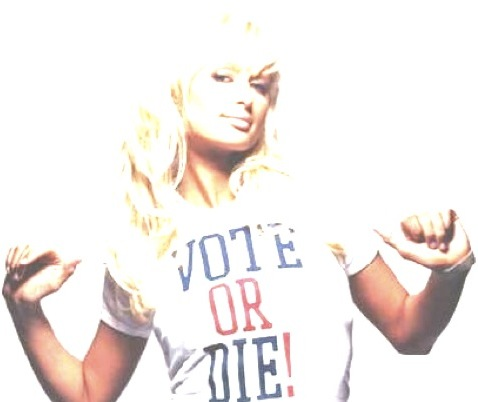
\includegraphics[height=.8\textheight]{vote}

    \end{columns}   

  \end{frame}
  %
  %
  
  % =========
  % = NOTES =
  % =========
  
  \section{Notes}
  
  %
  %
  \subsection{On computers}

  \begin{frame}[t]{A note on \red{computers}}
  
    \begin{columns}[T]

      \column{.4\textwidth}
      
      Despite what the general computing industry tells you, %
			computers are more than\\[1em]   

      \begin{itemize}
        \item Music players
        \item Facebook terminals
        \item Porn stashes
      \end{itemize}

      \column{.4\textwidth}

      
\includegraphics[width=\textwidth]{dilbert-porn}

    \end{columns}
  
      \vspace{1em}
      
      \begin{alertblock}{Important}
        This course requires that you \textbf{learn how to \emph{work}} with a computer. %
          \href{http://www.orbooks.com/catalog/program/}{Program or be programmed.}
      \end{alertblock}
      
  \end{frame}
  %
  %   


  %
  %
  \subsection{On software}

  \begin{frame}[t]{A note on \red{software}}
  
    \begin{columns}[T]

      \column{.4\textwidth}
      
      We will be using \red{Stata} throughout the semester.\\[1em]   

			Software details:
			
			\href{http://www.stata.com/}{stata.com}

      \column{.5\textwidth}

			\begin{center}
				\vspace{-2em}
				
\includegraphics[width=.5\textwidth]{icon-stata12}
			\end{center}
			
    \end{columns}
  
      \vspace{1em}
      
      \begin{alertblock}{Requirements}

				To operate Stata efficiently, you need

        \begin{itemize}
					\item to use a fairly recent computer with a bit of disk space
						% ... system requirements
        	\item to understand how files are organized on your hard drive
						% ... folder paths
					\item to type and `run' commands that follow a specific syntax
						% ... keyboard shortcuts
        \end{itemize}
        
      \end{alertblock}
      
  \end{frame}
  %
  %

  %
  %
  \subsection{On slides}
  %
  %
  
  \begin{frame}[t]{A note on \red{slides}}

    The course slides are absolutely insufficient to complete the %
		course requirements. You really need to do the readings.\\[1em]
		
		There is no way out of it.\\[1em]
      
    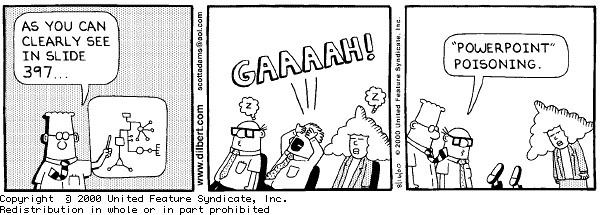
\includegraphics[width=\textwidth]{dilbert-ppt}

  \end{frame}
  %
  %

  %
  %
  \subsection{On emails}
  %
  %
  
  \begin{frame}[t]{A note on \red{emails}}

    \begin{alertblock}{Rules}
      \begin{enumerate}
        \item Start your email subject line with the ``\textbf{SRQM:}'' prefix.
        \item Describe the content of the email in the subject line.
        \item Attach your code and results to your question(s).
      \end{enumerate}
    \end{alertblock}
    
    \begin{block}{Google}
			\begin{itemize}
				\item This course requires \textbf{\href{http://mail.google.com/}{Google Mail}} %
					and \textbf{\href{http://docs.google.com/}{Google Docs}}
				\item This course assumes that you know how to use both tools
				\item Your \textbf{Sciences Po account} is actually a Google account
			\end{itemize}
    \end{block}

  \end{frame}
  %
  %

  \begin{frame}[t, plain]
    
    \vspace{.1\paperwidth}

    \begin{center}
      {%
      \Large \red{Welcome on board!}}\\[.1\paperwidth]
      
      \href{http://xkcd.com/552/}{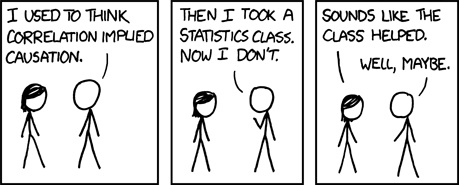
\includegraphics[height=4cm]{xkcd-correlation}%
      }
    \end{center}

  \end{frame}
  %
  %

	%
	%
  \section{Coursework}
	%
	%
	
  % \begin{frame}[t]{Coursework \red{for next week}}
  %
  % 		From this week onwards, you will need Stata to have been \textbf{set up for the course}. Listen carefully in class as we go through the procedure! Then, once you are set up, open Stata.\\[1em]%
  %
  %   \begin{block}{From Stata, type the line \code{in blue}}
  % 	    % \comm{Get the slides.}\\
  % 	    % \code{srqm\_get week1.pdf}\\
  %
  % 	    % \comm{Get the do-file.}\\
  % 	    % \code{srqm\_get week1.do}\\
  %
  % 			\comm{Open the do-file.}\\
  % 			\code{doedit code/week1}
  %   \end{block}
  %
  %   \begin{alertblock}{Homework}
  %     \begin{itemize}
  % 	       \item \textbf{Read the do-file} and execute its commands.
  % 	       \item \textbf{Practice} searching and describing variables.
  % 	       \item \textbf{Start thinking} about which dataset to analyse.
  %     \end{itemize}
  %   \end{alertblock}
  %
  % \end{frame}
  % %
  % %
	
\end{document}

